\documentclass{article}%
\usepackage{amsmath}
\usepackage{amsfonts}
\usepackage{amssymb}
\usepackage{graphicx}
\usepackage{tikz}
\usepackage{hyperref}%
\setcounter{MaxMatrixCols}{30}
%TCIDATA{OutputFilter=latex2.dll}
%TCIDATA{Version=5.00.0.2552}
%TCIDATA{CSTFile=40 LaTeX article.cst}
%TCIDATA{Created=Thursday, August 21, 2008 14:03:59}
%TCIDATA{LastRevised=Wednesday, October 01, 2014 12:46:33}
%TCIDATA{<META NAME="GraphicsSave" CONTENT="32">}
%TCIDATA{<META NAME="SaveForMode" CONTENT="1">}
%TCIDATA{<META NAME="DocumentShell" CONTENT="Standard LaTeX\Blank - Standard LaTeX Article">}
%TCIDATA{Language=American English}
\newtheorem{theorem}{Theorem}
\newtheorem{acknowledgement}[theorem]{Acknowledgement}
\newtheorem{algorithm}[theorem]{Algorithm}
\newtheorem{axiom}[theorem]{Axiom}
\newtheorem{case}[theorem]{Case}
\newtheorem{claim}[theorem]{Claim}
\newtheorem{conclusion}[theorem]{Conclusion}
\newtheorem{condition}[theorem]{Condition}
\newtheorem{conjecture}[theorem]{Conjecture}
\newtheorem{corollary}[theorem]{Corollary}
\newtheorem{criterion}[theorem]{Criterion}
\newtheorem{definition}[theorem]{Definition}
\newtheorem{example}[theorem]{Example}
\newtheorem{exercise}[theorem]{Exercise}
\newtheorem{lemma}[theorem]{Lemma}
\newtheorem{notation}[theorem]{Notation}
\newtheorem{problem}[theorem]{Problem}
\newtheorem{proposition}[theorem]{Proposition}
\newtheorem{remark}[theorem]{Remark}
\newtheorem{solution}[theorem]{Solution}
\newtheorem{summary}[theorem]{Summary}
\newenvironment{proof}[1][Proof]{\noindent\textbf{#1.} }{\ \rule{0.5em}{0.5em}}
\begin{document}

\title{CS 473 - Homework 4}
\author{Christopher Chapline}
\maketitle

\section{Problem 1}

\begin{proof}
    Let $E_1=0(10)*$ and let $E_2=(01)*0$.\\
    \\
    Basis: Let us first consider $w=0$. This is accepted by both $E_1$ and $E_2$ because the remainder of their
    expressions are closed over, meaning that they are not required for acceptance. Thus, our basis is satisfied.\\
    \\
    Induction: Let $w$ be a string that is accepted by $E_1$ and $E_2$. Assume that we append a $10$ to the end of the
    string. This will result in a string that is still accepted by both expressions. We know that $w$ is accepted by $E_1$
    based on the inductive hypothesis. Knowing this, we can say that $w10$ is accepted because it falls into the pattern of
    repetition specified by the Kleene closure of $(10)$. We also know that $w$ is accepted by $E_2$ by the inductive
    hypothesis. Knowing this, we can say that the last $0$ in $w10$ is the last zero in the expression $E_2$ and that the
    preceeding pattern of $01$ repetitions is captured by the Kleene closure of $01$.\\
    \\
    Thus, the expressions $E_1$ and $E_2$ accept the string $w10$.
\end{proof}

\section{Problem 2}

\begin{proof}
    Let $L_1$ and $L_2$ represent the languages accepted by $E_1=(\epsilon + 01)*$ and $E_2=(01)*$ respectively.\\
    \\
    Basis: Let $s$ be $\epsilon$. We know that $\epsilon(E*)$ is true for all expressions $E$. Thus, we can conclude
    that $\epsilon((\epsilon + 01)*)$ is true and that $\epsilon((01)*)$ is true. Our basis is satisfied.\\
    \\
    Induction: Let $w$ be a string in $L_1$ and $L_2$. The concatenation of the string $01$ onto $w$ would yield the string
    $w01$. This string is in both $L_1$ and $L_2$ because it represents the pattern $01$ which has been concatenated onto a
    string which is already in both languages, by the inductive hypothesis. Because both $E_1$ and $E_2$ represent closures
    over the pattern $01$, the string $w01$ is in $L_1$ and $L_2$.\\
    \\
\end{proof}

\section{Problem 3}

\begin{proof}
    Consider the subexpression $E_1 = (b0)*$. We must show the equivalence between $E_1$ and the following automaton:\\
    \\
    \begin{center}
        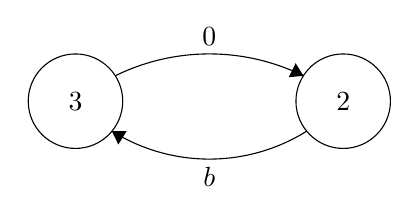
\begin{tikzpicture}[scale=0.2]
            \tikzstyle{every node}+=[inner sep=0pt]
            \draw [black] (17.3,-23.9) circle (3);
            \draw (17.3,-23.9) node {$3$};
            \draw [black] (34.3,-23.9) circle (3);
            \draw (34.3,-23.9) node {$2$};
            \draw [black] (31.989,-25.8) arc (-57.94807:-122.05193:11.662);
            \fill [black] (19.61,-25.8) -- (20.02,-26.65) -- (20.55,-25.8);
            \draw (25.8,-28.08) node [below] {$b$};
            \draw [black] (19.824,-22.289) arc (116.1997:63.8003:13.536);
            \fill [black] (31.78,-22.29) -- (31.28,-21.49) -- (30.84,-22.38);
            \draw (25.8,-20.4) node [above] {$0$};
        \end{tikzpicture}
    \end{center}\\
    \\
    Basis: Consider the empty string. The empty string will start in state $2$ and take no transitions, meaning it
    will stay in the same state. The expression $E_1$ will accept the string based on the definition of the Kleene
    closure.\\
    \\
    Induction: Let $w$ be a string that is accepted by $E_1$ and transitons back to state $2$ in the automaton. The
    concatenation of $b0$ onto $w$ will result in two transitions being taken from state $2$ (which is where $w$ takes
    us based on the inductive hypothesis) thus returning to state $2$. In the regular expression, this concatenation
    is performed on a string already accepted by $E_1$ (inductive hypothesis). This concatenation is accepted based upon
    the definition of the Kleene Closure.\\
    \\
    Thus, the strings accepted by $E_1$ start and end in the same state for the automaton.\\
    \\
\end{proof}

\begin{proof}
    Consider the subexpression $E_2 = (a1)*$. We must show equivalence between $E_2$ and the following automaton:\\
    \\
    \begin{center}
        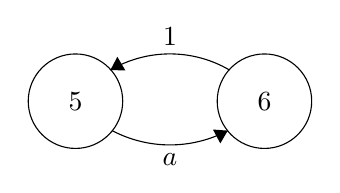
\begin{tikzpicture}[scale=0.2]
            \tikzstyle{every node}+=[inner sep=0pt]
            \draw [black] (15.1,-29.6) circle (3);
            \draw (15.1,-29.6) node {$5$};
            \draw [black] (27.1,-29.6) circle (3);
            \draw (27.1,-29.6) node {$6$};
            \draw [black] (24.775,-31.467) arc (-62.1647:-117.8353:7.87);
            \fill [black] (24.77,-31.47) -- (23.83,-31.4) -- (24.3,-32.28);
            \draw (21.1,-32.88) node [below] {$a$};
            \draw [black] (17.325,-27.617) arc (120.24033:59.75967:7.496);
            \fill [black] (17.32,-27.62) -- (18.27,-27.65) -- (17.76,-26.78);
            \draw (21.1,-26.1) node [above] {$1$};
        \end{tikzpicture}
    \end{center}\\
    \\
    Basis: Consider the empty string. The empty string will start in state $5$ and take no transitions, meaning it
    will stay in the same state. The expression $E_2$ will accept the string based on the definition of the Kleene
    closure.\\
    \\
    Induction: Let $w$ be a string that is accepted by $E_2$ and transitons back to state $5$ in the automaton. The
    concatenation of $a1$ onto $w$ will result in two transitions being taken from state $5$ (which is where $w$ takes
    us based on the inductive hypothesis) thus returning to state $5$. In the regular expression, this concatenation
    is performed on a string already accepted by $E_2$ (inductive hypothesis). This concatenation is accepted based upon
    the definition of the Kleene Closure.\\
    \\
    Thus, the strings accepted by $E_2$ start and end in the same state for the automaton.

\end{proof}

\begin{proof}
    We will now prove that the expression $(0(b0)*a1(a1)*b)*$ is equivalent to the following automaton:\\
    \\
    \begin{center}
        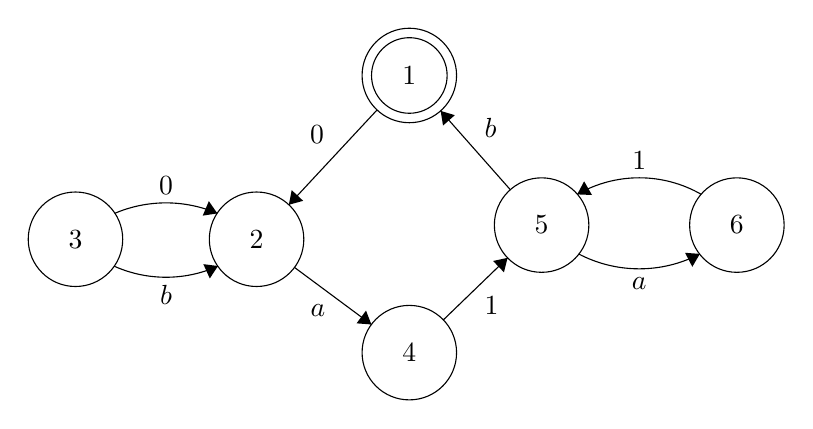
\begin{tikzpicture}[scale=0.2]
            \tikzstyle{every node}+=[inner sep=0pt]
            \draw [black] (41.9,-28.7) circle (3);
            \draw (41.9,-28.7) node {$5$};
            \draw [black] (54.3,-28.7) circle (3);
            \draw (54.3,-28.7) node {$6$};
            \draw [black] (33.5,-36.8) circle (3);
            \draw (33.5,-36.8) node {$4$};
            \draw [black] (33.5,-19.2) circle (3);
            \draw (33.5,-19.2) node {$1$};
            \draw [black] (33.5,-19.2) circle (2.4);
            \draw [black] (23.8,-29.6) circle (3);
            \draw (23.8,-29.6) node {$2$};
            \draw [black] (12.3,-29.6) circle (3);
            \draw (12.3,-29.6) node {$3$};
            \draw [black] (51.946,-30.534) arc (-62.41798:-117.58202:8.307);
            \fill [black] (51.95,-30.53) -- (51.01,-30.46) -- (51.47,-31.35);
            \draw (48.1,-31.98) node [below] {$a$};
            \draw [black] (44.157,-26.751) arc (119.93076:60.06924:7.902);
            \fill [black] (44.16,-26.75) -- (45.1,-26.79) -- (44.6,-25.92);
            \draw (48.1,-25.2) node [above] {$1$};
            \draw [black] (21.352,-31.305) arc (-65.80647:-114.19353:8.058);
            \fill [black] (21.35,-31.3) -- (20.42,-31.18) -- (20.83,-32.09);
            \draw (18.05,-32.51) node [below] {$b$};
            \draw [black] (14.79,-27.956) arc (113.09769:66.90231:8.31);
            \fill [black] (21.31,-27.96) -- (20.77,-27.18) -- (20.38,-28.1);
            \draw (18.05,-26.79) node [above] {$0$};
            \draw [black] (31.45,-21.39) -- (25.85,-27.41);
            \fill [black] (25.85,-27.41) -- (26.76,-27.16) -- (26.03,-26.48);
            \draw (28.12,-22.94) node [left] {$0$};
            \draw [black] (26.21,-31.39) -- (31.09,-35.01);
            \fill [black] (31.09,-35.01) -- (30.75,-34.13) -- (30.15,-34.94);
            \draw (27.7,-33.7) node [below] {$a$};
            \draw [black] (35.66,-34.72) -- (39.74,-30.78);
            \fill [black] (39.74,-30.78) -- (38.82,-30.98) -- (39.51,-31.7);
            \draw (38.72,-33.23) node [below] {$1$};
            \draw [black] (39.91,-26.45) -- (35.49,-21.45);
            \fill [black] (35.49,-21.45) -- (35.64,-22.38) -- (36.39,-21.72);
            \draw (38.24,-22.5) node [right] {$b$};
        \end{tikzpicture}
    \end{center}\\
    \\
    Basis: Consider the empty string, $w=\epsilon$. This input will result in the automaton taking no transitions
    and ending in an accepting state. Similarly, the empty string is in the language of any expression which has
    been closed over. Therefore, the empty string is in the language of the regular expression and the automaton.\\
    \\
    Induction: Let $w$ be a string accepted by $E$ and the automaton. Consider the concatenation of $0$, followed by
    zero or more repetitions of $b0$, $a1$, zero or more repetitions of $a1$, followedly lastly by a $b$. The $0$
    concatenated onto $w$ will take the automaton to state $2$.\\
    \\
    Because $w$ is accepted by the automataon, we know that we are starting the state $1$. The zero or more repetitions
    of $b0$ will return the automaton to state $2$ by the first lemma. The $a1$ will take the automaton from state $2$
    to state $5$. The zero or more repetitions of $a1$ will return the automaton to state $5$ by the second lemma. The
    $b$ following the $a1$ repetition will transition the automata back to state $1$, which means the string is accepted.\\
    \\
    Because $w$ is accepted by $E$ and $E$ is closed over, we can concatenate a string onto $w$. Provided that the string
    concatenated onto $w$ is accepted by the expression that is closed over, we know that that the regular expression accepts
    the concatenation. Assume $s=0 \phi a1 \alpha b$ where $\phi$ represents zero or more repetitions of $b0$ and $\alpha$
    represents zero or more repetitions of $a1$. The acceptance of $\phi$ and $\alpha$ follow from the first and second
    lemmas respectively. Assuming that $\phi$ and $\alpha$ accept their inputs and then rest of the string concatenated onto
    $w$ is formed correctly, the regular expression will accept the input.\\
    \\
\end{proof}

\section{Problem 4}

\begin{proof}
    We will first demonstrate that the subexpression $E_1=(01)*$ and the following automaton are equivalent:\\
    \\
    \begin{center}
        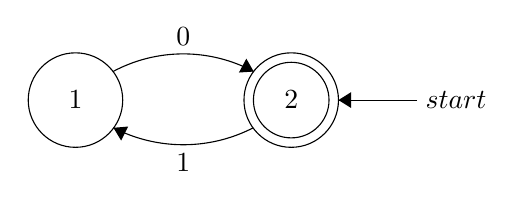
\begin{tikzpicture}[scale=0.2]
            \tikzstyle{every node}+=[inner sep=0pt]
            \draw [black] (32.4,-24.2) circle (3);
            \draw (32.4,-24.2) node {$2$};
            \draw [black] (32.4,-24.2) circle (2.4);
            \draw [black] (18.7,-24.2) circle (3);
            \draw (18.7,-24.2) node {$1$};
            \draw [black] (21.077,-22.39) arc (118.20527:61.79473:9.464);
            \fill [black] (30.02,-22.39) -- (29.55,-21.57) -- (29.08,-22.45);
            \draw (25.55,-20.77) node [above] {$0$};
            \draw [black] (29.986,-25.961) arc (-62.7541:-117.2459:9.69);
            \fill [black] (21.11,-25.96) -- (21.6,-26.77) -- (22.05,-25.88);
            \draw (25.55,-27.54) node [below] {$1$};
            \draw [black] (40.4,-24.2) -- (35.4,-24.2);
            \draw (40.9,-24.2) node [right] {$start$};
            \fill [black] (35.4,-24.2) -- (36.2,-24.7) -- (36.2,-23.7);
        \end{tikzpicture}
    \end{center}\\
    \\
    Basis: We will first consider the empty string. On the empty string, the automaton does not transition meaning that the
    automaton will end at state $2$, which is an accepting state. $E$ will accept the empty string because
    of the definition of the Kleene closure.\\
    \\
    Induction: Let $w$ be a string accepted by $E$ and the automaton. Consider the string $s=w10$. By the inductive hypothesis,
    we know that the automaton will start at state $2$. The sequence $01$ will transition the automaton to state $1$ and then
    back to state $2$. The automaton will accept this input. $E$ will also accept the input because the $10$ is a successive
    concatenation of the pattern $10$ which is closed over in $E$. We know that $w$ consists entirely of zero or more repetitions
    of $10$.\\
    \\
\end{proof}

\begin{proof}
    We will now prove that the expression $E=0(10)*0 ( 1(10)*0 )*$ equivalent to the following automaton:\\
    \\
    \begin{center}
        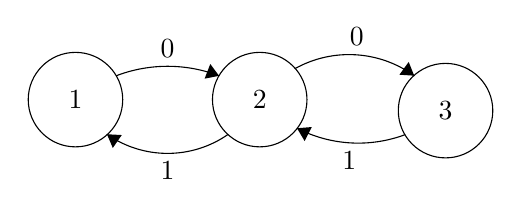
\begin{tikzpicture}[scale=0.2]
            \tikzstyle{every node}+=[inner sep=0pt]
            \draw [black] (23.3,-28.1) circle (3);
            \draw (23.3,-28.1) node {$1$};
            \draw [black] (35,-28.1) circle (3);
            \draw (35,-28.1) node {$2$};
            \draw [black] (46.8,-28.8) circle (3);
            \draw (46.8,-28.8) node {$3$};
            \draw [black] (25.876,-26.59) arc (110.98033:69.01967:9.143);
            \fill [black] (32.42,-26.59) -- (31.86,-25.84) -- (31.5,-26.77);
            \draw (29.15,-25.48) node [above] {$0$};
            \draw [black] (33,-30.303) arc (-55.03528:-124.96472:6.718);
            \fill [black] (25.3,-30.3) -- (25.67,-31.17) -- (26.24,-30.35);
            \draw (29.15,-32.02) node [below] {$1$};
            \draw [black] (37.236,-26.134) arc (119.14715:54.063:7.055);
            \fill [black] (44.81,-26.58) -- (44.46,-25.71) -- (43.87,-26.52);
            \draw (41.16,-24.7) node [above] {$0$};
            \draw [black] (44.234,-30.324) arc (-69.44452:-117.34533:8.472);
            \fill [black] (37.37,-29.92) -- (37.85,-30.73) -- (38.31,-29.84);
            \draw (40.69,-31.4) node [below] {$1$};
        \end{tikzpicture}
    \end{center}\\
    \\
    Basis: First consider the string $w=00$. Starting from the start state ($1$), $w$ will cause the automaton to transition to
    state $3$. This state is accepting. For $E$, the first $0$ corresponds to the $0$ at the start of the pattern and the second
    $0$ corresponds to the $0$ after the first $(10)*$ term. The string $w$ is in the language of $E$ because everything after the
    second $0$ is closed over, and is thus optional. This means that $E$ accepts $00$.\\
    \\
    Induction: Let $w=0\phi0\alpha$ where $\phi$ and $\alpha$ are sub-strings that are accepted by $(01)*$ and $(1(10)*0)*$
    respectively. There are several cases for addition into $w$:

    \begin{case}
        In this case, we insert a $10$ into $\phi$. This is still accepted by the automaton based on the lemma above. In other words,
        as long as the substring $\phi$ is still accepted by $(10)*$, then the regular expression will accept it and the automaton will
        still transition into an accepting state at the end. This follows from the inductive hypothesis and the lemma above.
    \end{case}

    \begin{case}
        Assume that we insert a $10$ into $\phi$. In this case, the automaton is already in an accepting state at the end of $w$. The
        insertion of a $10$ will result in the automaton translating from state $3$ to state $2$ and the back into state $3$, which is
        an accepting state. In the expression $E$, the addition will be handled by the surrounding elements in $1(10)*0$. This will yield
        acceptance by the expression $E$.
    \end{case}

    \begin{case}
        Assume that we insert a $1$ followed zero or more repetitions of $10$ and $0$. We know that $w$ is in the accepting state $3$ based
        upon the inductive hypothesis. Because of this, the insertion will have the effect of travleing from state $3$ to state $1$, then
        looping between states $1$ and $2$ for the number of repetitions of $10$, ending on state $2$ and will then transition to state $3$
        on the final $0$ and yield acceptance. In the expression, this insertion is handled by definition by the $(1(10)*0)$ sub-expression.
    \end{case}\\
    \\
    Because all three insertion cases will yield acceptance in both the automaton and the DFA, they accept the same language.
\end{proof}

\section{Problem 5}

\begin{proof}
    This proof follows directly from the the lemmas presented on slides $8$ and $9$ in class. Assuming that the first lemma
    is satisfied and the second lemma is satisfied with the remainder of the input, then the input string is accepted by the
    DFA and the regular expression.\\
    \\
\end{proof}

\section{Problem 6}

Recall that $R_{i,j}^k = R_{i,j}^{k-1} + R_{i,k}^{k-1}(R_{k,k}^{k-1})* + R_{k,j}^{k-1}$.\\
\\
The k-paths calculuation for this DFA follows:\\
\\
\subsection{The 0-paths:}\\
$R_{1,1}^0 = \epsilon$,
$R_{1,2}^0 = \emptyset$,
$R_{1,3}^0 = 0$\\
\\
$R_{2,1}^0 = \emptyset$,
$R_{2,2}^0 = \epsilon$,
$R_{2,3}^0 = 1$\\
\\
$R_{3,1}^0 = 1$,
$R_{3,2}^0 = 0$,
$R_{3,3}^0 = \epsilon$\\
\\
\subsection{The 1-paths:}\\
$R_{1,1}^1 = \epsilon$,
$R_{1,2}^1 = \epsilon$,
$R_{1,3}^1 = 0 + 00$\\
\\
$R_{2,1}^1 = \epsilon$,
$R_{2,2}^1 = \epsilon$,
$R_{2,3}^1 = 1 + 01$\\
\\
$R_{3,1}^1 = 1$,
$R_{3,2}^1 = 0 + 1$
$R_{3,3}^1 = \epsilon + 01$\\
\\
\subsection{The 2-paths:}\\
\\
$R_{1,1}^2 = \epsilon$,
$R_{1,2}^2 = \epsilon$,
$R_{1,3}^2 = 0 + 00 + 1+01$\\
\\
$R_{2,1}^2 = \epsilon$,
$R_{2,2}^2 = \epsilon$,
$R_{2,3}^2 = 1 + 01$\\
\\
$R_{3,1}^2 = 1 + 0$,
$R_{3,2}^2 = 0 + 1$,
$R_{3,3}^2 = \epsilon + 01 + (1 + 01)(\epsilon + 01)*(0 + 1)$\\
\\
\subsection{The 3-paths:}\\
\\
$R_{1,1}^3 = \epsilon + (1 + 0)(\epsilon + 01 + (1 + 01)(\epsilon + 01)*(0 + 1))*(0 + 00 + 1 + 01)$,
$R_{1,2}^3 = \epsilon + (1 + 01)(\epsilon + 01 + (1 + 01)(\epsilon + 01)*(0 + 1))*(0 + 1)$
$R_{1,3}^3 = (0 + 00 + 1 + 01) + (\epsilon + 01 + (1 + 01)(\epsilon + 01)*(0 + 1))$\\
\\
$R_{2,1}^3 = \epsilon + (1 + 01)(\epsilon + 01 + (1 + 01)(\epsilon + 01)*(0 + 1))*(1 + 0)$,
$R_{2,2}^3 = \epsilon + (0 + 1)(\epsilon + 01 + (1 + 01)(\epsilon + 01)*(0 + 1))*(1 + 01)$,
$R_{2,3}^3 = (1 + 01) + (\epsilon + 01 + (1 + 01)(\epsilon + 01)*(0 + 1))(\epsilon + 01 + (1 + 01)(\epsilon + 01)*(0 + 1))*(1 + 01)$\\
\\
$R_{3,1}^3 = (1 + 0) + (1 + 0)(\epsilon + 01 + (1 + 01)(\epsilon + 01)*(0 + 1))*(\epsilon + 01 + (1 + 01)(\epsilon + 01)*(0 + 1))$,
$R_{3,2}^3 = (0 + 1) + (0 + 1)(\epsilon + 01 + (1 + 01)(\epsilon + 01)*(0 + 1))*(\epsilon + 01 + (1 + 01)(\epsilon + 01)*(0 + 1))$,
$R_{3,3}^3 = (\epsilon + 01 + (1 + 01)(\epsilon + 01)*(0 + 1)) + (\epsilon + 01 + (1 + 01)(\epsilon + 01)*(0 + 1))(\epsilon + 01 + (1 + 01)
(\epsilon + 01)*(0 + 1))*(\epsilon + 01 + (1 + 01)(\epsilon + 01)*(0 + 1))$\\
\\
The final regular expression generated by k-paths is $(\epsilon + (0 + 1)(\epsilon + 01 + (1 + 01)(\epsilon + 01)*(0 + 1))*(1 + 01)) + (\epsilon + (1 + 01)(\epsilon + 01 + (1 + 01)(\epsilon + 01)*(0 + 1))*(0 + 1))$\\
\\
This regular expression is much, much longer and more difficult to read than $0(01 + 10)*0$. This is a standard pattern for regular
expressions generated through the k-paths expansion method. They generally create very long and very complex regular expressions
that are far from the optimal solution.
\end{document}
